Este capítulo aborda o modelo proposto neste trabalho de um sistema de arquivos distribuídos tolerante a falhas. Ele inicia com a visão geral da arquitetura do sistema apresentando detalhes do serviço de metadados, serviço de armazenamento, servidor e cliente. Em seguida é abordado as operações realizadas pelo sistema de arquivos distribuído proposto. Seguindo com o capítulo, é explanado como foi realizada a implementação do sistema de arquivos distribuído utilizando conceitos de RAID, focando especialmente nos serviços de metadados e de armazenamento, além dos clientes.


	\section{Arquitetura do sistema}
	
	A arquitetura do Sistema de Arquivos Distribuídos proposto neste trabalho é composto por um ou vários clientes comunicando-se com os servidores de metadados e de armazenamento, onde cada um está conectado através da Internet ou outra rede, como a Figura~\ref{fig:vis_sis} sintetiza. Neste sistema, cada servidor de armazenamento comporta-se da mesma forma como um disco rígido em um sistema RAID, armazenando distribuidamente as partes dos arquivos e/ou paridades associadas. \\
	
\begin{figure}[htb]
	\begin{center}
		
		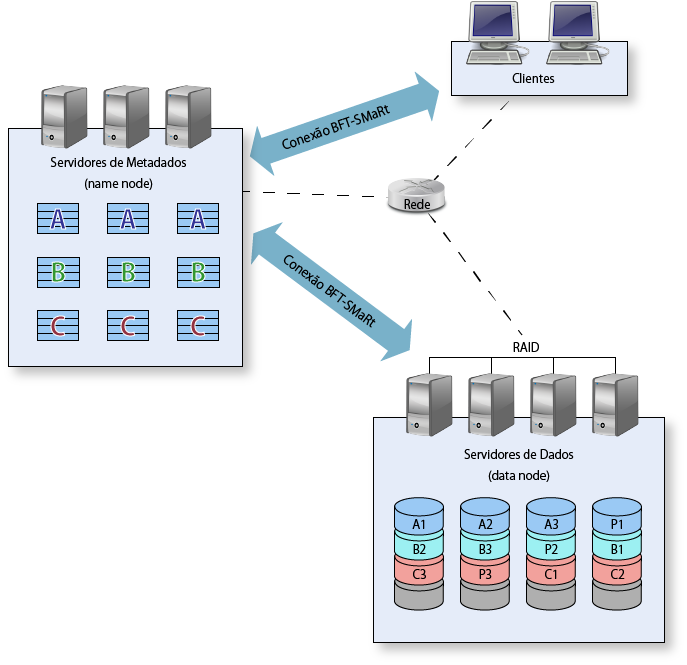
\includegraphics[clip,width=10.0cm]{images/visao_geral.png}
		\caption{Visão geral do sistema}
		\label{fig:vis_sis}
	\end{center}
\end{figure}

Em um sistema de arquivos local, normalmente os dados e metadados referentes ao arquivo são armazenados na mesma unidade de armazenamento. Entretanto, no caso de um sistema de arquivos distribuídos (SAD), os arquivos podem ser armazenados distribuidamente entre servidores distintos, ocasionando na necessidade de inserir metadados entre todos os servidores onde os arquivos estejam armazenados. Tal característica dificulta a recuperação de um arquivo em especifico, pois ela pode levar a uma busca completa em todos os servidores do sistema. Obviamente essa busca consome recursos operacionais, relativamente alta por se tratar de uma transmissão de rede.
   \\

%\begin{figure}[htb]
%	\begin{center}
		
%		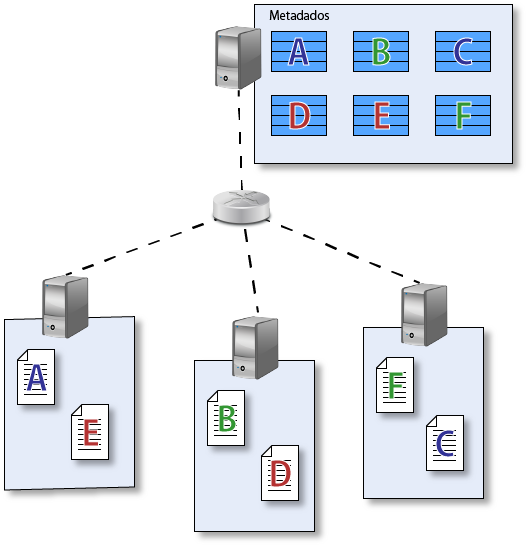
\includegraphics[clip,width=10.0cm]{images/image7.png}
%		\caption{\textit{Name node} e \textit{data node}}
%		\label{fig:namenode}
%	\end{center}
%\end{figure}

\subsection{Serviço de Metadados}
%Grupo de servidores que fazem o gerenciamento dos dados.\\

O sistema proposto utiliza o conceito de blocos. Cada bloco pode ser um conjunto de dados ou informações de paridade referentes a um único arquivo. O tamanho do bloco é determinado levando em consideração a quantidade de servidores de armazenamento ativos. Por exemplo, se houverem quatro servidores ativos, então o arquivo (independente de seu tamanho) será dividido em quatro blocos de tamanhos idênticos, caso seja necessário, o último bloco será preenchido com bits "0" até que o bloco alcance o tamanho dos outros blocos. Deste modo a quantidade de \textit{bytes} dos blocos é diretamente proporcional ao tamanho original do arquivo.
\\ 

O Serviço de metadados é composto pelos servidores, chamados de \textit{name nodes}, responsáveis por gerenciar os arquivos armazenados no sistema. Para tal utilizam-se dos metadados. No sistema proposto a data de criação, data da última modificação, data do último acesso, tamanho, identificador do bloco de dados e nome do servidor são considerados metadados. 
\\

Também é da responsabilidade do sistema de metadados gerenciar a comunicação entre cliente e servidores de armazenamento (ou  \textit{data nodes}). Utilizando-se das informações que indicam o estado atual do sistema (instantâneos de estado) e qual nível de RAID está sendo utilizado, o \textit{name node} deve decidir em quantos blocos de tamanho idêntico o arquivo deve ser dividido e em quais servidores de armazenamento cada bloco deve ser armazenado.
\\ 

O sistema está preparado para tratar os seguintes níveis de RAID, os quais foram explorados com maior profundidade no Capítulo 4. O nível de RAID que será executado deve ser informado no momento em que o serviço de metadado é inicializado.
\\

\begin{itemize}
	\item RAID 0 - fracionamento simples;
	\item RAID 1 - espelhamento;
	\item RAID 5 - fracionamento com paridade espalhada entre os discos do vetor.
\end{itemize}

O Serviço de metadados mantém na sua memória local a árvore de diretórios, a qual indica a localização lógica dos arquivos. Quando o serviço de metadados recebe uma solicitação proveniente do cliente para recuperar algum arquivo, primeiramente é realizada uma pesquisa na árvore de diretórios do cliente para identificar em qual diretório o arquivo encontra-se. Caso o arquivo seja encontrado, obtém-se seus metadados, sua localização física, a lista de todos os \textit{data nodes} que possuem os seus blocos.
\\

Devido sua propriedade como uma interface entre clientes e \textit{data nodes}, a ocorrência de alguma falha ou indisponibilidade de algum servidor degrada a execução do sistema, podendo até resultar na parada total do sistema. Assim, é de fundamental importância a elaboração de algum esquema para manter os \textit{name nodes} protegidos contra falhas ou queda total. No sistema proposto é utilizado a biblioteca BFT-SMaRt, a qual fornece tolerância a falha no serviço através de replicação por máquina de estado~\citep{bessani3}. 
\\

\subsection{Serviço de Armazenamento}
O Serviço de Armazenamento é composto pelo grupo de servidores responsáveis pelo armazenamento físico dos dados gerenciados pelo sistema de metadados. Também conhecido como \textit{data nodes}. No sistema proposto, o serviço de armazenamento não possui a necessidade de saber qual nível de RAID está sendo executado, pois a responsabilidade de manter o RAID consistente é toda do serviço de metadados. Desta forma, o serviço de armazenamento apenas se conecta a uma porta e fica aguardando algum cliente conectar-se a sua respectiva porta. Quando algum cliente conecta-se na porta do servidor, é realizado um \textit{handshake} preliminar, logo em seguida o cliente inicia a transferência dos dados que devem ser guardados pelo sistema de armazenamento. Ao fim da transferência o cliente fecha a conexão, enquanto o sistema de armazenamento indexa o arquivo recebido utilizando as informações adicionais que o serviço de metadados anexou ao arquivo. Com tais informações é possível saber o identificador tanto do arquivo quanto do cliente que o enviou. Tais dados adicionais são necessários para garantir que apenas o usuário dono dos dados enviados tenha acesso a eles, além de possibilitar identificar quais dados o cliente deseja receber de forma simples e eficiente.
\\

\subsection{Cliente}
O programa cliente executado no computador do usuário final do sistema. Para cada operação que deseje realizar, o programa cliente (doravante chamado Cliente) deve primeiramente comunicar-se com o serviço de metadados, o qual ou irá realizar a operação (no caso de operações envolvendo diretórios) ou informar com quais servidores de armazenamento o cliente deve se comunicar e quais blocos devem ser enviados para cada servidor (no caso de operações envolvendo arquivos).
\\

Após a comunicação inicial com o serviço de metadados, caso o cliente solicite pelo envio de arquivos ele deve iniciar a comunicação com os servidores de dados informados pelo serviço de metadados. Caso o serviço de metadado esteja utilizando o RAID 5, é o cliente quem fica responsável por calcular a paridade do arquivo, isto deve-se ao fato de que apenas o cliente conhece o arquivo. O procedimento para o cálculo da paridade é exemplificado na Figura~\ref{fig:img6}. Outra atribuição do cliente é fazer o particionamento do arquivo em blocos de tamanhos iguais, onde cada bloco será enviado para um dos servidores de dados informado pelo metadado, logo, o arquivo deve ser fragmentado de tal forma que cada servidor receba um bloco de dados, frisando que no caso do RAID 5 um dos blocos deve conter apenas informações de paridade previamente calculadas pelo cliente. 
\\

\begin{figure}[htb]
	\begin{center}
		
		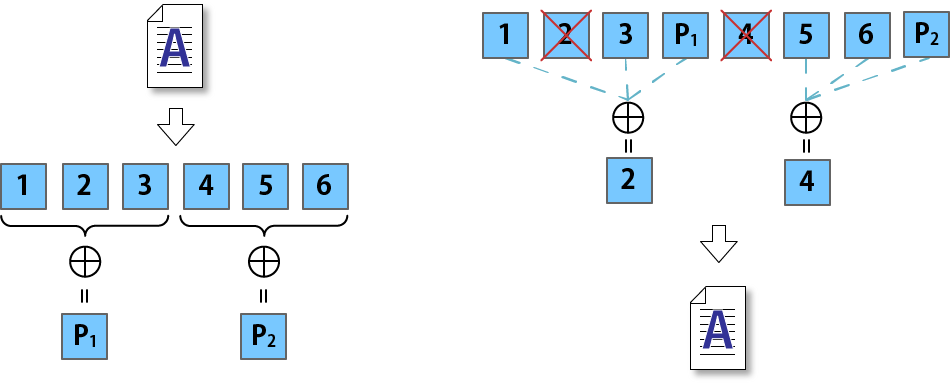
\includegraphics[clip,width=15.0cm]{images/image6.png}
		\caption{Geração de paridade}
		\label{fig:img6}
	\end{center}
\end{figure}

Caso a operação desejada pelo usuário final seja a de \textit{download}, o cliente deve coletar as informações de quais servidores possuem os blocos do arquivo almejado e quais as informações de identificação de cada bloco através do serviço de metadados. Com posse de tais informações, o cliente deve iniciar a comunicação com cada um dos servidores de dados apresentando a identificação de qual bloco cada servidor de dados deve enviar. Quando todos os servidores acabarem seus envios, o cliente deve usar os dados em sua posse para unir todos os blocos e recriar o arquivo desejado pelo usuário. Obviamente, esta descrição genérica da operação vai sofrer leves alterações dependendo de qual opção de RAID o serviço de metadados esteja utilizando. No caso do RAID 5 é possível que um dos blocos recebidos pelo cliente seja um bloco de paridade, nesse caso o cliente deve utilizar as informações dos outros blocos para determinar qual é o bloco de dados faltante e utilizar a paridade para recuperar tal bloco. A Figura~\ref{fig:img2} mostra um esquema simplificado da operação de recuperar um arquivo realizado pelo lado do cliente.
\\

\begin{figure}[htb]
	\begin{center}
		
		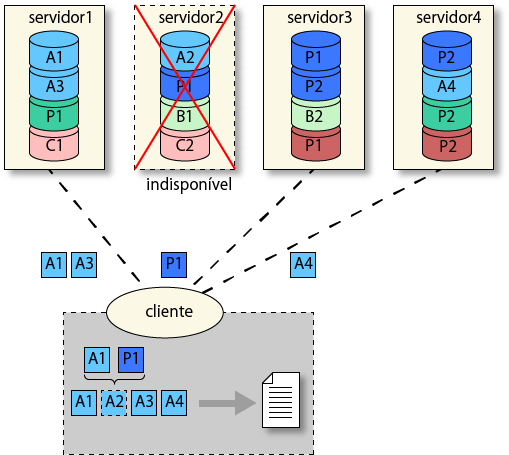
\includegraphics[clip,width=10.0cm]{images/image2.png}
		\caption{Recuperando um arquivo de uma falha}
		\label{fig:img2}
	\end{center}
\end{figure}

\section{Operações no Sistema de Arquivos Distribuídos}

Nesta seção serão apresentadas as operações básicas que o sistema de arquivos distribuídos (SAD) executa. Tais operações podem ser divididas em dois grupos dependendo das entidades envolvidas. O primeiro deles é entre cliente e servidor, composta por operações envolvendo solicitações de ações do cliente para o servidor. O segundo tipo são as operações que ocorrem entre servidores, voltadas para o gerenciamento do serviço sendo que este tipo de operações devem ocorrer de forma transparente para o cliente.
\\

\subsection{Cliente-Servidor}

É o conjunto de operações semelhantes as que são implementadas em um sistema de arquivos local, aquele que é integrado na maioria dos sistemas operacionais centralizados. Composto pelas operações sobre arquivos ou pastas, e suas execuções ocorrerem entre cliente e o serviço de metadados ou armazenamento.
\\

\subsubsection{Criar arquivo}

Operação realizada inicialmente entre o cliente e o serviço de metadados. Nesse primeiro momento o cliente informa ao \textit{name node} que deseja criar um novo arquivo e em qual diretório ele deve ser criado, além de enviar os metadados do arquivo que pretende criar. Com posse dessas informações e de qual RAID está operando, o serviço de metadados processa e transmite para o cliente para quais servidores do serviço de armazenamento os blocos do arquivo devem ser enviados e qual a identificação de cada bloco. O processamento de tais informações é diretamente influenciado pelo estado atual do sistema, o serviço de metadados leva em consideração a disponibilidade de cada servidor do serviço de armazenamento e o quanto de espaço livre em disco que cada um possui.
\\

A segunda parte da operação é realizada entre o cliente e os servidores do serviço de armazenamento. Após a comunicação com o serviço de metadados, o cliente sabe para quantos \textit{data nodes} o seu arquivo será enviado, desta forma, o cliente fragmenta o arquivo de forma que cada servidor receba um bloco de tamanho uniforme. Caso o sistema esteja usando o RAID 5, o cliente ainda deve calcular o bloco de paridade do arquivo e enviar para um dos \textit{data nodes}.
\\

\subsubsection{Criar diretório}

Operação realizada exclusivamente entre o cliente e o serviço de metadados. Nessa operação o cliente informa ao \textit{name node} que deseja criar um diretório, passando como metadados apenas o nome do novo diretório e o nome de seu diretório pai. Com tais informações, o serviço de metadados primeiramente verifica se já existe um diretório com o mesmo nome no diretório pai informado, em caso negativo ele atualiza a árvore de diretório do cliente. No caso de já existir um diretório com mesmo nome, o cliente é informado e o novo diretório não é criado.
\\

\subsubsection{Abrir arquivo}

Operação realizada inicialmente entre o cliente e o serviço de metadados. Nesse primeiro momento o cliente informa ao \textit{name node} que deseja abrir um arquivo, para tal, o cliente deve fornecer o nome do arquivo e o nome do diretório onde ele está salvo. A primeira ação do serviço de metadados é verificar se o arquivo de fato existe no diretório informado, em caso positivo ele ainda deve verificar se o cliente possui acesso ao arquivo. No caso do cliente possuir acesso, o serviço de metadados verifica em quantos blocos o arquivo foi dividido e em quais servidores do serviço de armazenamento cada bloco foi armazenado. Após coletar tais informações, o serviço de metadados informa ao cliente quais servidores de dados ele, o cliente, deve se comunicar e o identificador de cada bloco. Para o caso de o arquivo não existir no diretório informado ou do cliente não possuir permissão de acesso para tal arquivo, o serviço de metadados deve enviar uma mensagem de erro informando a indisponibilidade do arquivo solicitado. 
\\

A segunda parte da operação é realizada entre o cliente e os servidores do serviço de armazenamento. Após a comunicação com o serviço de metadados, o cliente sabe em quais servidores os blocos de seu arquivo estão armazenados. Desta forma, o cliente inicia a comunicação com cada servidor informado. A comunicação procede da seguinte forma: o cliente informa o identificador do bloco que deseja receber, enquanto que o \textit{data node} apenas verifica a existência do bloco informado. Em caso positivo, o bloco é enviado para o solicitante. Enquanto que no caso negativo, uma mensagem de erro alertando sobre a inexistência do bloco solicitado. Repare que o serviço de metadados não realiza nenhuma operação de controle de acesso sobre o bloco.
\\

A terceira parte da operação é realizada exclusivamente pelo cliente. Nesta última parte o cliente é responsável por unir todos os blocos recebidos e recriar o arquivo almejado.  Vale ressaltar que essa operação sofre variações dependo do RAID sendo utilizado. Para o caso do RAID 5, um dos blocos recebido pelo cliente pode ser um bloco de paridade, nesse caso, antes de recriar o arquivo o cliente deve utilizar as informações de paridade contidas em tal bloco para recuperar o bloco faltante. Para os outros níveis de RAID o cliente apenas recriar o arquivo utilizando os blocos recebidos.
\\

\subsubsection{Abrir diretório}

Operação realizada exclusivamente entre o cliente e o serviço de metadados. Nessa operação o cliente informa ao \textit{name node} que deseja abrir um diretório, passando como parâmetros apenas os nomes do novo diretório almejado e do diretório atual. A primeira ação do serviço de metadados é verificar a existência do diretório solicitado, em caso positivo, o serviço também verifica se o cliente possui permissão de acesso e se o diretório está livre. Caso todas as validações sejam positivas, o servidor muda o diretório atual do cliente para o diretório solicitado. Caso algum problema seja detectado uma mensagem de erro é disparada para o cliente, sem alterar seu diretório atual.
\\

\subsubsection{Deletar arquivo}

Operação realizada primeiramente entre o cliente e o serviço de metadados. Nessa operação o cliente informa ao \textit{name node} que deseja deletar um arquivo, em seguida deve informar o nomes do arquivo e do diretório onde ele está armazenado. Com tais informações, o serviço de metadados percorre a árvore de diretórios em busca do diretório requisitado, caso seja encontrado, inicia nele uma pesquisa pelo arquivo informado. Se o arquivo for encontrado, o serviço de metadados verifica se o cliente possui permissão de acesso ao arquivo e se ele não está em estado de bloqueio, em caso positivo o arquivo é deletado da lista dos metadados e a árvore de diretório do cliente é atualizada. Antes de finalizar a conexão o serviço de metadados informa ao cliente os dados sobre os blocos que compõe o arquivo.
\\

A segunda parte da operação é realizada entre o cliente e serviço de armazenamento. O cliente inicia uma conexão com cada servidor de dados onde um bloco do seu arquivo está armazenado e o informa que o referido bloco deve ser deletado.
\\

\subsubsection{Deletar diretório}

Operação realizada exclusivamente entre o cliente e o serviço de metadados. Nessa operação o cliente informa ao \textit{name node} que deseja deletar um diretório, passando apenas o nome do diretório almejado. A primeira ação do serviço de metadados é verificar a existência do diretório solicitado. Em caso positivo o serviço de metadados também verifica se este diretório é vazio. Se neste diretório existir algum arquivo ou subdiretório a operação falha. Caso contrario o serviço de metadados continua com a verificação: se o cliente possui permissão de acesso e se o diretório está livre. Caso todas as validações sejam positivas o serviço de metadados deleta o diretório. Em seguida o serviço de metadados atualiza a árvore de diretórios do cliente.
\\

\subsubsection{Fechar um arquivo aberto}

Operação realizada exclusivamente entre o cliente e o serviço de metadados. Nessa operação o cliente informa ao \textit{name node} que deseja fechar um arquivo. Primeiramente o serviço de metadados verifica se existe algum arquivo aberto pelo cliente, caso exista, é apresentado ao cliente a lista de arquivos abertos para que ele selecione qual ele deseja fechar. Sabendo qual arquivo deve ser fechado o serviço de metadados libera o acesso ao \textit{lock} do arquivo, desta forma fechando o arquivo. Para o caso de o cliente não ter nenhum arquivo aberto é emitida uma mensagem de erro explicativa para o usuário.
\\

\subsubsection{Fechar diretório}

Operação realizada exclusivamente entre o cliente e o serviço de metadados. Nessa operação o cliente informa ao \textit{name node} que deseja fechar um diretório atual. Primeiramente o serviço de metadados verifica se o diretório atual é o diretório raiz, caso seja, o cliente é informado que não pode fechar o diretório raiz. Caso não seja o raiz, o diretório atual é atualizado para o diretório pai do antigo diretório atual.
\\

\subsubsection{Editar um arquivo}

Operação realizada inicialmente entre o cliente e o serviço de metadados. Nesse primeiro momento o cliente informa ao \textit{name node} que deseja editar um arquivo, para tal, o cliente deve fornecer o nome do arquivo. Em posse do nome do arquivo o serviço de metadados verifica sua existência no diretório corrente, em caso positivo ainda é preciso confirmar se o arquivo já está aberto. Verificado que o arquivo encontra-se fechado as informações sobre o arquivo são passados para o cliente. Com tais informações, a operação que o cliente realiza é a exclusão do antigo arquivo seguida da criação de um novo (ou seja, a atualização do antigo arquivo). Tais operações são realizadas como descrito previamente, entretanto, com a diferença que o usuário não precisa informar o nome do arquivo pois ele é criado com o mesmo nome do antigo.
\\

\subsubsection{Renomear um arquivo}
Operação realizada entre o cliente e o serviço de metadados. Nessa operação o cliente informa ao \textit{name node} que deseja renomear um arquivo, além de fornecer o nome do arquivo que deve ser renomeado ele também deve informar o novo nome. Primeiramente o serviço de metadados procura pelo arquivo informado no diretório corrente, caso o arquivo seja encontrado ainda é necessário que o serviço de metadados verifique se o cliente possui permissão de acesso ao arquivo e se o mesmo está fechado. Caso o arquivo esteja fechado e o cliente tenha permissão de acesso, o arquivo é, enfim, renomeado com o novo nome.
\\

\subsubsection{Renomear Diretório}

Operação realizada exclusivamente entre o cliente e o serviço de metadados. Nessa operação o cliente informa ao \textit{name node} que deseja renomear o diretório, além de fornecer o nome do diretório que deve ser renomeado e o seu novo nome. Primeiramente o serviço de metadados percorre a árvore de diretórios em busca do nome fornecido. Caso seja encontrado, o diretório é renomeado com o novo nome fornecido pelo cliente. Por fim, o metadado referente a última modificação do diretório é atualizado.
\\

%	\subsection{Servidor-Servidor}
%	São operações realizadas entre os \textit{name nodes} e os \textit{data nodes}, com função de gerenciamento do Sistema de Arquivos Distribuídos.

%	\subsubsection{Receber arquivo criado}

%	Na operação de criar arquivo, o \textit{name node} define quais \textit{data nodes} vão ser utilizados para armazenar os fragmentos de arquivo a ser criado, calculando a melhor forma para distribuir igualmente a carga entre os \textit{data nodes}. Dessa forma, além de informar ao cliente quais são os servidores para os quais deve enviar os dados, também deve avisar aos \textit{data nodes} que um cliente irá iniciar uma transferência de dados.

%	\subsubsection{Apagar arquivo deletado}

%	Além das ações entre o \textit{name node} e o cliente explanadas na subseção anterior, para efetivamente deletar um arquivo, o \textit{name node} também....

%	Deleta os dados pertencentes ao arquivo solicitado para exclusão.

%	\subsubsection{Transferir dados entre servidores}

%	Transferência de arquivos entre \textit{data nodes}.

